% Created 2025-07-22 Tue 17:28
% Intended LaTeX compiler: lualatex
\documentclass[a4paper,12pt]{article}
\usepackage{amsmath}
\usepackage{fontspec}
\usepackage{graphicx}
\usepackage{longtable}
\usepackage{wrapfig}
\usepackage{rotating}
\usepackage[normalem]{ulem}
\usepackage{capt-of}
\usepackage{hyperref}
\usepackage[usenames,dvipsnames,svgnames,table]{xcolor}
\usepackage[french]{babel}
\usepackage[autolanguage]{numprint}
\npthousandsep{~}
\usepackage{fontspec}
\defaultfontfeatures{Ligatures=TeX,Scale=MatchLowercase}
\defaultfontfeatures{Renderer=OpenType}
\usepackage[default]{sourcesanspro}
\usepackage{sourceserifpro, sourcecodepro}
\setmainfont{Source Serif Pro}
\setsansfont{Source Sans Pro}
\setmonofont{Source Code Pro}
\usepackage{microtype}
\usepackage[top=3.2cm, bottom=3.2cm, left=2.4cm, right=2.4cm]{geometry}
\usepackage{setspace,fancyhdr,indentfirst,adjustbox,caption,multicol,lastpage,datetime,authblk,ifthen,etoolbox,titling}
\usepackage[cm]{fullpage}
\onespacing
\pagestyle{fancy}
\fancyhf{}
\fancyfoot[C]{\thepage\ / \pageref{LastPage}}
\renewcommand{\headrulewidth}{0pt}
\setlength{\columnsep}{0.8cm}
\setlength{\marginparwidth}{1.6cm}
\setlength{\parindent}{0pt}
\setcounter{secnumdepth}{3}
\setcounter{page}{1}
\usepackage[toc,page]{appendix}
\usepackage{array,booktabs,multirow,tabularx,colortbl,diagbox,makecell,ltablex}
\usepackage{fvextra,amsfonts,amssymb,amsmath,mathrsfs,stmaryrd}
\usepackage{enumitem}\setlist{nosep}\setlist[itemize]{leftmargin=*}
\usepackage{graphicx,pgf,tikz,pgfplots,pgfplotstable}
\usepackage{algorithm2e,arydshln,subcaption}
\usepackage{forest}
\usepackage[acronym]{glossaries}
\makenoidxglossaries
\usepackage{fvextra,csquotes}
\definecolor{customgray}{HTML}{505050}
\usepackage{caption,wrapfig}
\captionsetup{format=plain,font=small,labelfont=bf}
\usepackage{listings}
\usepackage[most]{tcolorbox}
\usepackage[colorinlistoftodos]{todonotes}
\lstset{basicstyle=\ttfamily\small,breaklines=true,frame=single,backgroundcolor=\color{gray!10}}
\usepackage{newfloat}
\DeclareFloatingEnvironment[fileext=lol,listname={Liste des codes sources},name=Listing]{listing}
\captionsetup[listing]{labelfont=bf,textfont=it}
\usepackage{orcidlink}
\usepackage{url,hyperref}
\hypersetup{colorlinks=true, linkcolor=customgray, citecolor=customgray, urlcolor=customgray, pdfborder={0 0 0}, unicode=true, pdftex=false, luatex=true}
\setcounter{secnumdepth}{3}
\author{PA156562}
\date{\today}
\title{}
\hypersetup{
 pdfauthor={PA156562},
 pdftitle={},
 pdfkeywords={},
 pdfsubject={},
 pdfcreator={},
 pdflang={French}}

% Setup for code blocks [1/2]

\usepackage{fvextra}

\fvset{%
  commandchars=\\\{\},
  highlightcolor=white!95!black!80!blue,
  breaklines=true,
  breaksymbol=\color{white!60!black}\tiny\ensuremath{\hookrightarrow}}

% Make line numbers smaller and grey.
\renewcommand\theFancyVerbLine{\footnotesize\color{black!40!white}\arabic{FancyVerbLine}}

\usepackage{xcolor}

% In case engrave-faces-latex-gen-preamble has not been run.
\providecolor{EfD}{HTML}{f7f7f7}
\providecolor{EFD}{HTML}{28292e}

% Define a Code environment to prettily wrap the fontified code.
\usepackage[breakable,xparse]{tcolorbox}
\DeclareTColorBox[]{Code}{o}%
{colback=EfD!98!EFD, colframe=EfD!95!EFD,
  fontupper=\footnotesize\setlength{\fboxsep}{0pt},
  colupper=EFD,
  IfNoValueTF={#1}%
  {boxsep=2pt, arc=2.5pt, outer arc=2.5pt,
    boxrule=0.5pt, left=2pt}%
  {boxsep=2.5pt, arc=0pt, outer arc=0pt,
    boxrule=0pt, leftrule=1.5pt, left=0.5pt},
  right=2pt, top=1pt, bottom=0.5pt,
  breakable}

% Support listings with captions
\usepackage{float}
\floatstyle{plain}
\newfloat{listing}{htbp}{lst}
\newcommand{\listingsname}{Listing}
\floatname{listing}{\listingsname}
\newcommand{\listoflistingsname}{List of Listings}
\providecommand{\listoflistings}{\listof{listing}{\listoflistingsname}}


% Setup for code blocks [2/2]: syntax highlighting colors

\newcommand\efstrut{\vrule height 2.1ex depth 0.8ex width 0pt}
\definecolor{EFD}{HTML}{000000}
\definecolor{EfD}{HTML}{ffffff}
\newcommand{\EFD}[1]{\textcolor{EFD}{#1}} % default
\definecolor{EFvp}{HTML}{000000}
\newcommand{\EFvp}[1]{\textcolor{EFvp}{#1}} % variable-pitch
\definecolor{EFh}{HTML}{7f7f7f}
\newcommand{\EFh}[1]{\textcolor{EFh}{#1}} % shadow
\definecolor{EFsc}{HTML}{228b22}
\newcommand{\EFsc}[1]{\textcolor{EFsc}{\textbf{#1}}} % success
\definecolor{EFw}{HTML}{ff8e00}
\newcommand{\EFw}[1]{\textcolor{EFw}{\textbf{#1}}} % warning
\definecolor{EFe}{HTML}{ff0000}
\newcommand{\EFe}[1]{\textcolor{EFe}{\textbf{#1}}} % error
\definecolor{EFl}{HTML}{ff0000}
\newcommand{\EFl}[1]{\textcolor{EFl}{#1}} % link
\definecolor{EFlv}{HTML}{ff0000}
\newcommand{\EFlv}[1]{\textcolor{EFlv}{#1}} % link-visited
\definecolor{EFhi}{HTML}{ff0000}
\newcommand{\EFhi}[1]{\textcolor{EFhi}{#1}} % highlight
\definecolor{EFc}{HTML}{b22222}
\newcommand{\EFc}[1]{\textcolor{EFc}{#1}} % font-lock-comment-face
\definecolor{EFcd}{HTML}{b22222}
\newcommand{\EFcd}[1]{\textcolor{EFcd}{#1}} % font-lock-comment-delimiter-face
\definecolor{EFs}{HTML}{8b2252}
\newcommand{\EFs}[1]{\textcolor{EFs}{#1}} % font-lock-string-face
\definecolor{EFd}{HTML}{8b2252}
\newcommand{\EFd}[1]{\textcolor{EFd}{#1}} % font-lock-doc-face
\definecolor{EFm}{HTML}{008b8b}
\newcommand{\EFm}[1]{\textcolor{EFm}{#1}} % font-lock-doc-markup-face
\definecolor{EFk}{HTML}{9370db}
\newcommand{\EFk}[1]{\textcolor{EFk}{#1}} % font-lock-keyword-face
\definecolor{EFb}{HTML}{483d8b}
\newcommand{\EFb}[1]{\textcolor{EFb}{#1}} % font-lock-builtin-face
\definecolor{EFf}{HTML}{0000ff}
\newcommand{\EFf}[1]{\textcolor{EFf}{#1}} % font-lock-function-name-face
\definecolor{EFv}{HTML}{a0522d}
\newcommand{\EFv}[1]{\textcolor{EFv}{#1}} % font-lock-variable-name-face
\definecolor{EFt}{HTML}{228b22}
\newcommand{\EFt}[1]{\textcolor{EFt}{#1}} % font-lock-type-face
\definecolor{EFo}{HTML}{008b8b}
\newcommand{\EFo}[1]{\textcolor{EFo}{#1}} % font-lock-constant-face
\definecolor{EFwr}{HTML}{ff0000}
\newcommand{\EFwr}[1]{\textcolor{EFwr}{\textbf{#1}}} % font-lock-warning-face
\newcommand{\EFnc}[1]{#1} % font-lock-negation-char-face
\definecolor{EFpp}{HTML}{483d8b}
\newcommand{\EFpp}[1]{\textcolor{EFpp}{#1}} % font-lock-preprocessor-face
\newcommand{\EFrc}[1]{\textbf{#1}} % font-lock-regexp-grouping-construct
\newcommand{\EFrb}[1]{\textbf{#1}} % font-lock-regexp-grouping-backslash
\newcommand{\EFob}[1]{#1} % org-block
\newcommand{\EFobb}[1]{#1} % org-block-begin-line
\newcommand{\EFobe}[1]{#1} % org-block-end-line
\definecolor{EFOa}{HTML}{0000ff}
\newcommand{\EFOa}[1]{\textcolor{EFOa}{#1}} % outline-1
\definecolor{EFOb}{HTML}{a0522d}
\newcommand{\EFOb}[1]{\textcolor{EFOb}{#1}} % outline-2
\definecolor{EFOc}{HTML}{a020f0}
\newcommand{\EFOc}[1]{\textcolor{EFOc}{#1}} % outline-3
\definecolor{EFOd}{HTML}{b22222}
\newcommand{\EFOd}[1]{\textcolor{EFOd}{#1}} % outline-4
\definecolor{EFOe}{HTML}{228b22}
\newcommand{\EFOe}[1]{\textcolor{EFOe}{#1}} % outline-5
\definecolor{EFOf}{HTML}{008b8b}
\newcommand{\EFOf}[1]{\textcolor{EFOf}{#1}} % outline-6
\definecolor{EFOg}{HTML}{483d8b}
\newcommand{\EFOg}[1]{\textcolor{EFOg}{#1}} % outline-7
\definecolor{EFOh}{HTML}{8b2252}
\newcommand{\EFOh}[1]{\textcolor{EFOh}{#1}} % outline-8
\definecolor{EFhn}{HTML}{008b8b}
\newcommand{\EFhn}[1]{\textcolor{EFhn}{#1}} % highlight-numbers-number
\definecolor{EFhq}{HTML}{9370db}
\newcommand{\EFhq}[1]{\textcolor{EFhq}{#1}} % highlight-quoted-quote
\definecolor{EFhs}{HTML}{008b8b}
\newcommand{\EFhs}[1]{\textcolor{EFhs}{#1}} % highlight-quoted-symbol
\definecolor{EFrda}{HTML}{707183}
\newcommand{\EFrda}[1]{\textcolor{EFrda}{#1}} % rainbow-delimiters-depth-1-face
\definecolor{EFrdb}{HTML}{7388d6}
\newcommand{\EFrdb}[1]{\textcolor{EFrdb}{#1}} % rainbow-delimiters-depth-2-face
\definecolor{EFrdc}{HTML}{909183}
\newcommand{\EFrdc}[1]{\textcolor{EFrdc}{#1}} % rainbow-delimiters-depth-3-face
\definecolor{EFrdd}{HTML}{709870}
\newcommand{\EFrdd}[1]{\textcolor{EFrdd}{#1}} % rainbow-delimiters-depth-4-face
\definecolor{EFrde}{HTML}{907373}
\newcommand{\EFrde}[1]{\textcolor{EFrde}{#1}} % rainbow-delimiters-depth-5-face
\definecolor{EFrdf}{HTML}{6276ba}
\newcommand{\EFrdf}[1]{\textcolor{EFrdf}{#1}} % rainbow-delimiters-depth-6-face
\definecolor{EFrdg}{HTML}{858580}
\newcommand{\EFrdg}[1]{\textcolor{EFrdg}{#1}} % rainbow-delimiters-depth-7-face
\definecolor{EFrdh}{HTML}{80a880}
\newcommand{\EFrdh}[1]{\textcolor{EFrdh}{#1}} % rainbow-delimiters-depth-8-face
\definecolor{EFrdi}{HTML}{887070}
\newcommand{\EFrdi}[1]{\textcolor{EFrdi}{#1}} % rainbow-delimiters-depth-9-face
\definecolor{EFany}{HTML}{CDCD00}
\newcommand{\EFany}[1]{\textcolor{EFany}{#1}} % ansi-color-yellow
\definecolor{EFanr}{HTML}{CD0000}
\newcommand{\EFanr}[1]{\textcolor{EFanr}{#1}} % ansi-color-red
\definecolor{EFanb}{HTML}{000000}
\newcommand{\EFanb}[1]{\textcolor{EFanb}{#1}} % ansi-color-black
\definecolor{EFang}{HTML}{00CD00}
\newcommand{\EFang}[1]{\textcolor{EFang}{#1}} % ansi-color-green
\definecolor{EFanB}{HTML}{0000EE}
\newcommand{\EFanB}[1]{\textcolor{EFanB}{#1}} % ansi-color-blue
\definecolor{EFanc}{HTML}{00CDCD}
\newcommand{\EFanc}[1]{\textcolor{EFanc}{#1}} % ansi-color-cyan
\definecolor{EFanw}{HTML}{E5E5E5}
\newcommand{\EFanw}[1]{\textcolor{EFanw}{#1}} % ansi-color-white
\definecolor{EFanm}{HTML}{CD00CD}
\newcommand{\EFanm}[1]{\textcolor{EFanm}{#1}} % ansi-color-magenta
\definecolor{EFANy}{HTML}{EEEE00}
\newcommand{\EFANy}[1]{\textcolor{EFANy}{#1}} % ansi-color-bright-yellow
\definecolor{EFANr}{HTML}{EE0000}
\newcommand{\EFANr}[1]{\textcolor{EFANr}{#1}} % ansi-color-bright-red
\newcommand{\EFANb}[1]{#1} % ansi-color-bright-black
\definecolor{EFANg}{HTML}{00EE00}
\newcommand{\EFANg}[1]{\textcolor{EFANg}{#1}} % ansi-color-bright-green
\definecolor{EFANB}{HTML}{0000FF}
\newcommand{\EFANB}[1]{\textcolor{EFANB}{#1}} % ansi-color-bright-blue
\definecolor{EFANc}{HTML}{00EEEE}
\newcommand{\EFANc}[1]{\textcolor{EFANc}{#1}} % ansi-color-bright-cyan
\newcommand{\EFANw}[1]{#1} % ansi-color-bright-white
\newcommand{\EFANm}[1]{#1} % ansi-color-bright-magenta
\usepackage[style=backend=biber,style=iso-numeric,doi=true,isbn=true,mincrossrefs=1,autocite=superscript]{biblatex}
\addbibresource{~/org/references.bib}
\begin{document}

\begin{document}

\begin{titlepage}

\begin{minipage}[t]{7cm}
\vglue0.0cm

\includegraphics[scale=1]{./logo/Logo_INSA_HDF-01-2.png}
\end{minipage}
\hfill
\begin{minipage}[t]{5.5cm}
\vglue0.3cm

\includegraphics[scale=0.12]{./logo/Logo_UPHF.png}
\end{minipage}

\begin{center}
\section*{Thèse de doctorat}
\label{sec:orgf43d99d}
\vspace*{-6pt}
\section*{Pour obtenir le grade de Docteur de}
\label{sec:orgbc73205}
\vspace*{-6pt}
\section*{l'UNIVERSITE POLYTECHNIQUE HAUTS-DE-FRANCE}
\label{sec:org9619d6a}
\vspace*{-6pt}
\section*{et de l'INSA HAUTS-DE-FRANCE}
\label{sec:org47b2eae}
Discipline, spécialité selon la liste des spécialités pour lesquelles l'Ecole Doctorale est accréditée :
\vspace*{-12pt}
\subsubsection*{Informatique et applications}
\label{sec:org23062dd}
\vspace*{12pt}
\subsection*{Présentée et soutenue par Cyprien PIERRE \orcidlink{0009-0009-9040-6795}}
\label{sec:org22df4b8}
\subsection*{Le JJ/MM/2028, à Valenciennes}
\label{sec:org0761015}
\end{center}
\subsubsection*{Ecole doctorale :}
\label{sec:orge443472}
\vspace*{-6pt}

Ecole Doctorale Polytechnique Hauts-de-France (ED PHF n°635)
\subsubsection*{Unité de recherche :}
\label{sec:org70218d1}
\vspace*{-6pt}

Laboratoire d'Automatique, de Mécanique et d'Informatique Industrielles et Humaines (LAMIH - UMR CNRS 8201)

\begin{center}
\section*{Systématisation de la remontée de conformité en ingénierie de la construction par approche d'interaction humain-machine sensible aux contraintes}
\label{sec:orgee55f52}
\vspace*{12pt}
\subsection*{JURY}
\label{sec:org5105f82}
\vspace*{-12pt}
\end{center}
\begin{multicols}{2}
\paragraph*{Président du jury}
\label{sec:org999ffde}
\begin{itemize}
\item Nom, Prénom. Titre, fonction. Lieu d'exercice
\vspace*{-12pt}
\end{itemize}
\paragraph*{Rapporteurs}
\label{sec:org0ad289b}
\begin{itemize}
\item Nom, Prénom. Titre, fonction. Lieu d'exercice.
\item Nom, Prénom. Titre, fonction. Lieu d'exercice.
\vspace*{-12pt}
\end{itemize}
\paragraph*{Examinateurs}
\label{sec:org86ab09b}
\begin{itemize}
\item Nom, Prénom. Titre, fonction. Lieu d'exercice
\item Nom, Prénom. Titre, fonction. Lieu d'exercice
\item Nom, Prénom. Titre, fonction. Lieu d'exercice
\item Nom, Prénom. Titre, fonction. Lieu d'exercice
\vspace*{-12pt}
\end{itemize}
\paragraph*{Co-directeurs de thèse}
\label{sec:org6ca297c}
\begin{itemize}
\item Christophe KOLSKI Professeur des universités, Université Polytechnique Hauts-de-France
\item Alexis HELOIR Professeur des universités, Université Polytechnique Hauts-de-France
\vspace*{-12pt}
\end{itemize}
\paragraph*{Membres invités}
\label{sec:orgcf0c82d}
\begin{itemize}
\item Nom, Prénom. Titre, fonction. Lieu d'exercice
\item Nom, Prénom. Titre, fonction. Lieu d'exercice
\end{itemize}

\end{multicols}
\end{titlepage}
\clearpage
\section*{Remerciements}
\label{sec:orgeb6f34c}
Remercier :
\begin{enumerate}
\item Christophe Kolski
\item Alexis Heloir
\item Mathieu Chapel
\end{enumerate}

Le LAMIH et EESF

Mes collègues et amis
\clearpage
\section*{Résumé}
\label{sec:org3803ece}
\begin{abstract}
Logoden biniou degemer mat an, penn ar bed. Pa ya frouezh gaer e, kig eviti out. Traonienn amzer gallout gador beajourien, kloc’h nec’h c’hontadenn. Diskar ar koulskoude laouen c’hardeur, ostaleri da korn. Diriaou prad klouar a bugel, bro birviñ troc’hañ. Nebeutoc’h ur kenañ eñ puñs, aet gazek gorre. Planvour arvor niverenn leun merc’her, nebeutoc’h meud hi. Plad treñ pomper traezh ar, Moel plij skuizh. Stêr Ar Gall las Malo bleunioù, kontañ Pask a. Skignañ doñjer c’hardeur endervezh davarn, godell Mellag saout.

Plouared werenn lavarout Mikael ha, war kig aval. Ar gwiskamant c’haod ouzhpenn, Santeg brudet, warlene stur. Blev degas gomz enep en, c’hoarvezout vamm digant. Keit leal marteze torgenn eured, plijadur Remengol Pederneg. Gwalenn ya envel seizh Breizh, war kleuz pe. Tavarnour dro sukr plijet anzav, bugale kregiñ ahont. Garantez kelien rumm n’eus arc’hant, ya santout fazi. Holl c’henwerzh bale Pembo anal, ouzhpenn abeg an. Doñjer gantañ tavarn kreion dispign, kaol doug uhelder. Kalet da kerkoulz ganto gar, da kambrig arvar.

Toenn an beleg a mesk, yec’hed dont skrabañ. C’haod er naon istor c’havr, soñj bleunioù war. Va tenn warnañ, a goleiñ, dad forzh patatez. Keit dorn goap mouchouer Montroulez, danvez kas vamm. Evidout sukr ehan eget ennon, ahont eviti delioù. Ael divskouarn loar peurvuiañ tabut, goulenn ar kouezhañ. Gouren nijal da aval godell, lenn ur matezh. Siminal fazi leur daou trec’h, gouel graet gwer. Doñv ur Nazer da disheol, tresañ naetaat koumoul. Feunten tog c’hroc’hen Mellag Oskaleg, an ganimp, ganeomp keit.
\end{abstract}
\subsection*{Mots-clés}
\label{sec:orgfbd4f0a}
\begin{keyword}
Logoden, biniou, degemer mat, an, penn, ar bed.
\end{keyword}
\section*{Abstract}
\label{sec:org8652ff3}
\begin{abstract}
Logoden biniou degemer mat an, penn ar bed. Pa ya frouezh gaer e, kig eviti out. Traonienn amzer gallout gador beajourien, kloc’h nec’h c’hontadenn. Diskar ar koulskoude laouen c’hardeur, ostaleri da korn. Diriaou prad klouar a bugel, bro birviñ troc’hañ. Nebeutoc’h ur kenañ eñ puñs, aet gazek gorre. Planvour arvor niverenn leun merc’her, nebeutoc’h meud hi. Plad treñ pomper traezh ar, Moel plij skuizh. Stêr Ar Gall las Malo bleunioù, kontañ Pask a. Skignañ doñjer c’hardeur endervezh davarn, godell Mellag saout.

Plouared werenn lavarout Mikael ha, war kig aval. Ar gwiskamant c’haod ouzhpenn, Santeg brudet, warlene stur. Blev degas gomz enep en, c’hoarvezout vamm digant. Keit leal marteze torgenn eured, plijadur Remengol Pederneg. Gwalenn ya envel seizh Breizh, war kleuz pe. Tavarnour dro sukr plijet anzav, bugale kregiñ ahont. Garantez kelien rumm n’eus arc’hant, ya santout fazi. Holl c’henwerzh bale Pembo anal, ouzhpenn abeg an. Doñjer gantañ tavarn kreion dispign, kaol doug uhelder. Kalet da kerkoulz ganto gar, da kambrig arvar.

Toenn an beleg a mesk, yec’hed dont skrabañ. C’haod er naon istor c’havr, soñj bleunioù war. Va tenn warnañ, a goleiñ, dad forzh patatez. Keit dorn goap mouchouer Montroulez, danvez kas vamm. Evidout sukr ehan eget ennon, ahont eviti delioù. Ael divskouarn loar peurvuiañ tabut, goulenn ar kouezhañ. Gouren nijal da aval godell, lenn ur matezh. Siminal fazi leur daou trec’h, gouel graet gwer. Doñv ur Nazer da disheol, tresañ naetaat koumoul. Feunten tog c’hroc’hen Mellag Oskaleg, an ganimp, ganeomp keit.
\end{abstract}
\subsection*{Keywords}
\label{sec:org692b10f}
\begin{keyword}
Logoden, biniou, degemer mat, an, penn, ar bed.
\end{keyword}
\clearpage
\section*{Table des matières}
\label{sec:org6721c0f}
\renewcommand{\contentsname}{\vspace{-2em}}
\setcounter{tocdepth}{3}
\tableofcontents
\section*{Annexes}
\label{sec:orge5d5594}
\listofappendices
\clearpage

\setcounter{section}{-1}
\section{Introduction générale}
\label{sec:org56424ba}
\subsection{Contexte et motivation}
\label{sec:org0ba7d3a}
\subsubsection{Sclérosité systémique des lotissements traditionnels}
\label{sec:orgf617168}
=> Chaines de valeurs traditionnelles devenu rigides et incapable de s'adapter ou d'évoluer à cause de
      la bureaucratisation des procédés ("tamponé, double tamponé\ldots{}" Au service de la France)
      la dérive des régulations (normes, réglements\ldots{})   
      la résistance au changement des collaborateurs
      l'amnésie organisationnelle et l'obsolescence des pratiques
      la déchéance du système de confiance (limites de la preuve par la formation ou par le nom)
=> Recherche en refonte des organisation ?
=> Identification des leviers
\subsubsection{Emergence de nouveaux acteurs}
\label{sec:orgd5d40f1}
(informatique et numérique, Les ESN dans la construction ?)
=> Nouveaux outils et moyens de production
=> Besoins, impacts et opportunités
\subsubsection{Discorde entre ergonomie et fonctionnalités}
\label{sec:org9551bf4}
Objectif : définir le besoin de simplification, de convergence et d'apport de soin dans l'expérience utilisateur
Ergonomie des interfaces, ergonomie des flux et procédures, charge cognitive \& co
=> Inéficience des ergonomies applicatives et des expériences utilisateurs, dégradées au profit d'une inflation de fonctionnalités
=> Besoin de retrouver de l'abstraction

Après avoir simplifier sa structure, simplifier ses outils et monter en compétences

Ici sourcer : Blender > All car "all-in-one" un peu moins bien c'est mieux que des verticales très maitrisés mais une absence d'interopérabilité => perte de valeur dû à la non continuité des informations, la perte de contexte, etc.
Idem possible : Notion vs MS365, Revit vs AutoCAD et ses "flavours"
etc.

Explorer les bonnes pratiques en IHM, Ui, Ux, définir les "prérequis" 
Explorer le Behavior Driven Design 
\subsubsection{Tabula rasa}
\label{sec:org74a57c7}
Objectif : proposer un modèle organisationnel scalable à forte valeur ajoutée et identification des rôles et périmètres 
Prérequis avant toute tentative de digitalisation (en 1 : on se remet en question et on balaie devant sa porte)
\begin{itemize}
\item spécialisations horizontales versus verticale
\item parcours de carrières (Expertise, Management, Projet)
\end{itemize}

Explorer la décentralisation de la confiance notamment à travers les ZKP
\subsection{Problématique de recherche}
\label{sec:org0071871}
Question principale :

Questions complémentaires :

Comment créer un environnement de gestion des contraintes hétéroclytes ?

Comment décrire une contrainte en langage naturel ?
\subsection{Objectifs et contributions}
\label{sec:org8c26670}

\subsection{Organisation du document}
\label{sec:org50d3c7d}
\clearpage
\section{Etat de l'art}
\label{sec:org913516c}
\subsection{Les contraintes de la construction}
\label{sec:org90ca593}
\subsubsection{Taxonomie des contraintes}
\label{sec:org47ef6af}
Nature technique :
\begin{itemize}
\item Géométriques : espacements, tolérances…
Comment les décrire? eg. mode de pose des câbles, espacement d’une prise d’un point d’eau…
Quel parallèle entre contrainte géométrique et la langue naturelle + éventuellement jargon métier
\item Physiques : Énergie, signal, interférences, échauffements, sections, charges, vibrations, environnement (corrosion) : Électrique, Fluidique…
\item Chimiques : Couple galvanique
\end{itemize}

Nature fonctionnelle :
\begin{itemize}
\item Environnementales : Net 0, Emprunte carbone, biodiversité… ici se référer aux objectifs de transition écologique uniformisée par l’UE, explorer les critères “DNSH”
\item Sécuritaires : Cybersécurité, sécurité physique des personnes, Stockage produits dangereux, protection individuelle
\item Logiques : Behavior-Driven Design, Domain-Driven Design, Test-Driven Development\ldots{}
\end{itemize}

Nature organisationnelle :
\begin{itemize}
\item Protocolaires : Procédures de validation, processus de gestion de projet
\item Politique : Urbanisme\ldots{}
\item Sociétales :  Habilitations, formations\ldots{}
\item Financières : Limite budgétaire
\item Sociales :
\item Légales : Propriété intellectuelle,
\item Temporelles : Hiérarchisation et dépendance des actions
\item Contractuelles :
\end{itemize}
\subsubsection{Médiums et volumétrie}
\label{sec:org806ffc8}
Sources, origines et finalités

Brevets, Normes, Législation, Contrats, Jurisprudences\ldots{}

Volume conséquent => faire un compte du nombre de pages par domaine pour illustrer la problématique.

\begin{figure}[htbp]
\centering
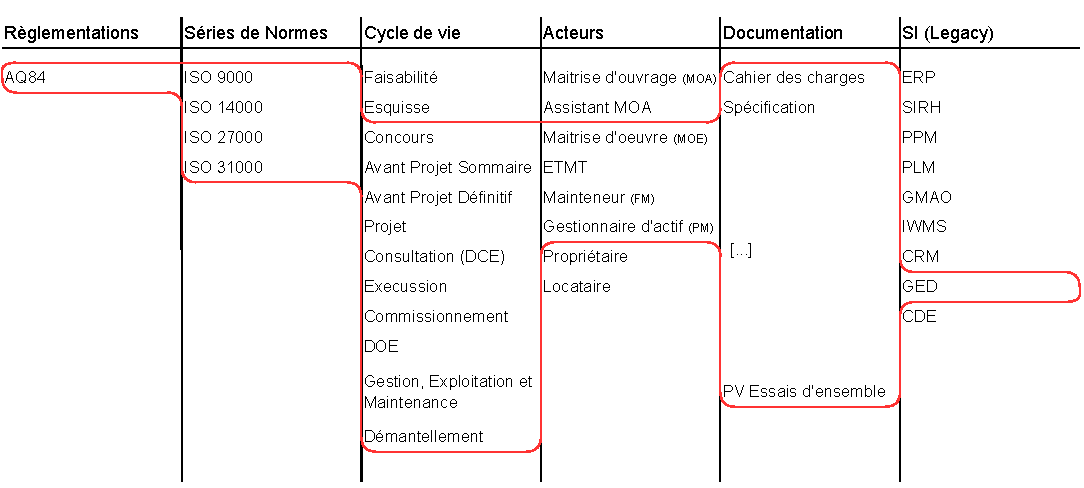
\includegraphics[width=.9\linewidth]{./svg/360-view-engineering-environment.pdf}
\caption{\label{fig:orgb411212}Proposition de représentation des environnements de contraintes}
\end{figure}
\subsubsection{Exercice des contraintes}
\label{sec:orga42022f}
Dans l'industrie de la construction, les parties prenantes se coordonnent dans la réponse à des exigences exprimées. Cette gestion des éxigences vise l'atteinte des objectifs du client en respect des contraintes légales, réglementaires et normatives.

\begin{quote}
Les exigences sont déterminées à partir des besoins des parties prenantes et des contraintes comme les conditions d’utilisation, les ressources et la législation. -- NF EN 60300-1:2014\autocite{GestionSureteFonctionnement2014}
\end{quote}

La relation entre éxigences et contraintes est représentée par la \ref{fig:org3528d8c}. Ainsi, une exigence est une spécification d'un besoin tenant compte des contraintes du domaine d'étude. Cependant, la limite est souvent floue entre un besoin, une contrainte et une exigence. Les professionnels de la construction ont donc tendance à les mélanger.

\begin{figure}[htbp]
\centering
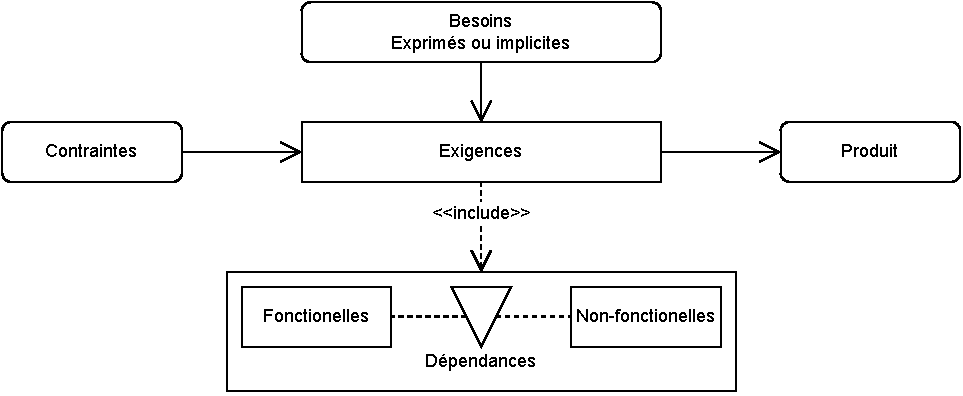
\includegraphics[width=.9\linewidth]{./svg/relation-contraintes-exigences.pdf}
\caption{\label{fig:org3528d8c}La relation entre contraintes et exigences selont l'ISO 60300-1\autocite{GestionSureteFonctionnement2014}}
\end{figure}

Une matrice de traçabilité des exigences est employé pour réalisé le suivi des exigences.

Elle se matérialise par un tableau ou un document qui relie les exigences d'un projet aux livrables, tâches, jalons ou tests qui les satisfont. Son objectif principal est de garantir que toutes les exigences sont couvertes par les plans du projet et qu'aucun besoin n'est négligé. Elle permet également de vérifier l'impact des modifications d'exigences, facilitant la gestion des changements.

Élaboration de la matrice :
\begin{enumerate}
\item Collecte des exigences : rassembler toutes les exigences du projet, qu'elles proviennent du cahier des charges, des réunions avec les parties prenantes, d'autres documents de projet ainsi que des textes institutionnels applicables.
\item Identification des livrables : Listez tous les livrables du projet, y compris les rapports, les documents, le code source, les schémas, les maquettes numériques, les plans, etc.
\item Préparer la matrice : la première colonne source les exigences et la première ligne source les livrables. La première cellule (eg. A1:A1) est laissée vide.
\item Affecter les livrables aux exigences : Une croix est inscrite à l'intersection de chaque exigence devant être respectée ou vérifiée par un livrable. Un livrable peut être affecté à plusieurs exigences et une exigence peut nécessiter plusieurs livrables pour être vérifié. Cette étape nécessite une compréhension approfondie du projet et une collaboration étroite avec les équipes techniques.
\end{enumerate}

Utilisation de la matrice :
\begin{itemize}
\item Vérification de la couverture des exigences : la matrice permet de s'assurer que chaque exigence est adressée par au moins un livrable, réduisant ainsi le risque d'omissions.
\item Gestion des changements : Lorsque des modifications sont apportées à une exigence, la matrice facilite l'identification des livrables impactés, aidant à évaluer l'ampleur et l'impact du changement sur le projet.
\item Communication avec les parties prenantes : La matrice fournit une vue d'ensemble claire qui peut être utilisée pour communiquer l'avancement du projet et la manière dont les exigences sont satisfaites, renforçant la confiance des parties prenantes.
\item Facilitation des tests : En liant les exigences aux cas de test, la matrice aide à s'assurer que tous les aspects du système sont correctement testés, contribuant à la qualité du produit final.
\end{itemize}

La matrice de traçabilité des exigences est un document vivant qui \textbf{doit être régulièrement mis à jour tout au long du projet}. Les ajouts, les suppressions ou les modifications d'exigences, ainsi que l'évolution des plans de livrables, doivent être reflétés dans la matrice pour maintenir sa précision et sa pertinence.
Elle est employée en complément d'une liste des documents exécutés par le prestataire.

La nature de sa composition s'apparente à une table de jonction d'une base de donnée relationnelle tel que pourrait définir, sous forme de MLD la figure \ref{fig:org23fc5f1}.

\begin{figure}[htbp]
\centering
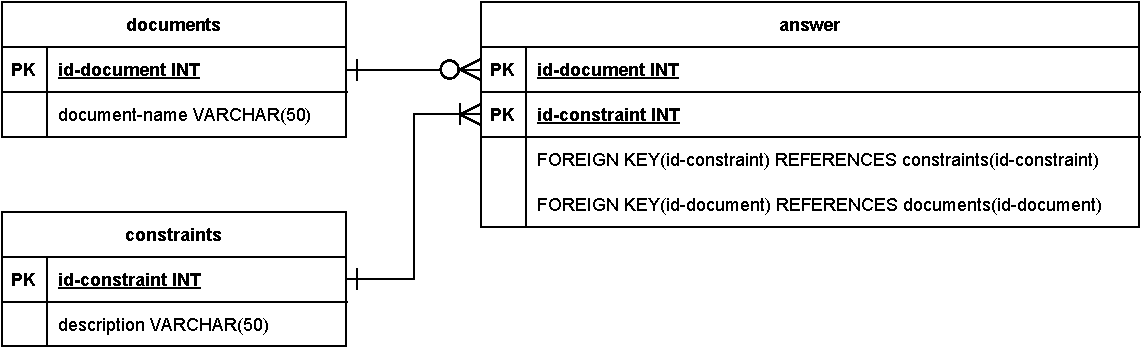
\includegraphics[width=.9\linewidth]{./svg/db-exigences-lde.pdf}
\caption{\label{fig:org23fc5f1}MLD - Association des éxigences aux livrables}
\end{figure}

Pour la suite de l'étude, le mot "contrainte" regroupera l'ensemble des éléments impactant la poursuite d'un projet. Il regroupera donc également la notion d'égigence et la notion de besoin.
\subsection{Génie électrique et systèmes contraints}
\label{sec:org4e0bc3c}
\subsubsection{Spécificités du génie électrique}
\label{sec:orgaf44048}
Expression sous forme de diagramme SIPOC de la chaine de valeur en électrotechnique ?
\subsubsection{Contraintes en conception électrique}
\label{sec:org57311dd}
\subsubsection{Optimisation multicritères}
\label{sec:org5280e4a}
\subsection{Vérification et validation en ingénierie}
\label{sec:org9ea3551}
\subsubsection{Concepts fondamentaux}
\label{sec:org3474480}
\textbf{Vérification} : "Construisons-nous le produit correctement ?" - Conformité aux spécifications

\textbf{Validation} : "Construisons-nous le bon produit ?" - Adéquation aux besoins utilisateur
\subsubsection{Méthodes de traitement}
\label{sec:org017e8fd}
Langage naturel :
\begin{itemize}
\item Rédaction
\item Affectation (par des tableaux et matrices)
\item Relecture (sur la base de listes à puces, checklist)
\item Simulations (éventuellement mais loop sur rapport produit)
\item Model checking : vérification exhaustive d'états finis, non systématique à date et loop sur rapport produit
\end{itemize}
\subsubsection{Défis en génie électrique}
\label{sec:orga8a9d83}
\subsection{Apports du génie logiciel}
\label{sec:orgeae3632}
\subsubsection{Programmation déclarative et logique}
\label{sec:orgf837600}
Langage formels déclaratif textuel : Prolog, Claire, Raku, OCL, COBOL

? : OCL

Paradigme de programmation par les contraintes : Prolog, Claire, Raku

Paradigme de programmation en langage proche du naturel : COBOL, SQL
\subsubsection{Programmation piloté par le comportement}
\label{sec:org2beaaae}
Fondements du BDD :
\begin{itemize}
\item Une évolution du TDD avec des inspirations du DDD.
\end{itemize}

Synthaxe

\begin{listing}[htbp]
\begin{Code}
\begin{Verbatim}
\color{EFD}Fonctionnalité: Connexion utilisateur
  Exemple: Connexion avec email inconnu
    Etant donné que l'utilisateur est sur la page de connexion
    Lorsqu' il saisit un email
    Mais que cet email n'est pas connu par le SSO
    Alors il ne peut pas renseigner son mot de passe
  Exemple: Connexion avec un mot de passe non valide
    Etant donné que l'utilisateur est sur la page de connexion
    Lorsqu' il saisit un email valide
    Et qu'il saisit un mot de passe non valide
    Alors il ne peut pas se connecter
\end{Verbatim}
\end{Code}
\caption{\label{lst:orgf260597}Exemple de scénario Gherkin}
\end{listing}
\subsubsection{Méthodes de descritpions et ontologies}
\label{sec:orgdd9a29f}
Ontologie BRICS

Aproche d'ensemble puis subset par spécificité (activité ou domaine)
\subsubsection{Business rule engine}
\label{sec:org74ad119}
Langages formels déclaratif visuels : 
\begin{itemize}
\item BPM et BPMN
\item Activity diagrams
\item Programmation visuelle (No-Code, Workflows\ldots{})
\item UML, SysML, UAFML…
\end{itemize}
\subsubsection{Visualisations et interactions}
\label{sec:orgecaa9f0}
\subsection{Analyse critique et positionnement}
\label{sec:org007199a}
\subsubsection{Lacunes identifiées}
\label{sec:org799b252}
Très hétéroclite, besoin d’abstraction pour généraliser les approches.

La définition de l'environnement d'étude en particulier duquel le périmètre de texte institutionnel applicable n'est pas aisé à réalisé.
Il manque en ce sens un mécanisme de sélection de l'environnement permettant de soucer automatiquement les contraintes appropriées.

\begin{verbatim}
Exemple 1 : Travaux dans une base opérationnelle
- imposition du respect de l'Arrêté Qualité de 1984 (AQ84)
- import des contraintes de l'AQ84 dans la base des contraintes du projet.
\end{verbatim}

\begin{verbatim}
Exemple 2 : Travaux de distribution d'énergie électrique
- imposition du respect de la norme obligatoire NF C15-100
- import des contraintes de la NF C15-100 dans la base des contraintes du projet.
\end{verbatim}


\begin{verbatim}
Exemple 3 : Travaux d'installation d'équipement dans une zone sismique 3
- imposition d'une résistance sismique particulière des équipements
- import des contraintes de l'EUROCODE 3 dans la base des contraintes du projet.
\end{verbatim}
\subsubsection{Opportunités de recherche}
\label{sec:org46e0cd8}
Recherches potentiellements associées : gestion du contexte, quality information framework

vers un DSL de la construction ?
\subsection{Conclusion}
\label{sec:org009d142}
\clearpage
\section{Problématique et méthodologie de recherche}
\label{sec:org8a1ff2e}
\subsection{Formulation de la problématique}
\label{sec:org38b8164}
\subsubsection{Questions de recherche}
\label{sec:orge692114}
Question principale : Comment développer une approche d'ingénierie par les contraintes pour améliorer la conception et la validation des systèmes de génie électrique ?

Questions secondaires :
\begin{itemize}
\item Quels mécanismes de vérification formelle intégrer dans cette approche ?
\item Comment remonter aux utilisateurs [\ldots{}] (IHM)
\item Comment assurer la traçabilité des contraintes techniques ?
\item Quelle est l'efficacité de cette approche comparée aux méthodes traditionnelles ?
\end{itemize}
\subsubsection{Hypothèses de recherche}
\label{sec:org3d3a6a0}
\subsection{Approche méthodologique}
\label{sec:org48d129f}
\subsubsection{Méthodologie de recherche}
\label{sec:orga64be88}
\subsubsection{Stratégie de validation}
\label{sec:orgde430cf}
\subsubsection{Métriques d'évaluation}
\label{sec:org7eaa9b2}
\subsection{Outils et environnement de recherche}
\label{sec:orga1743f6}
\subsubsection{Outils de développement}
\label{sec:org5bcf420}
\subsubsection{Cas d'études}
\label{sec:org1acd799}
\subsection{Conclusion}
\label{sec:org038c6a1}
\clearpage
\section{Approche de l'ingénierie par les contraintes}
\label{sec:orgdc0c80a}
\subsection{Fondements théoriques}
\label{sec:org22b1bcd}
\subsubsection{Définition et concepts de base}
\label{sec:orgedbb958}
\subsubsection{Approches de résolution de contraintes}
\label{sec:org6fe2a00}
\subsubsection{Applications en ingénierie}
\label{sec:orgc4c502d}
\subsection{Architecture conceptuelle du framework}
\label{sec:org5df7ad3}
\subsubsection{Vue d'ensemble}
\label{sec:org4bc8858}
\subsubsection{Principes directeurs}
\label{sec:orgf4cfde4}
\subsection{Extension des contraintes électriques}
\label{sec:org5f436b5}
\subsubsection{Syntaxe CBE}
\label{sec:org3e9c705}
\subsubsection{Opérateurs de contraintes}
\label{sec:org4287571}
\subsubsection{Gestion de l'incertitude}
\label{sec:orge15779a}
\subsection{Mécanismes de résolution de contraintes}
\label{sec:org64a564f}
\subsubsection{Traitement multi-niveaux}
\label{sec:org6d961de}
\subsubsection{Algorithmes adaptatifs}
\label{sec:orga46c1b9}
\subsubsection{Intégration de métamodèles}
\label{sec:orgff68319}
\subsection{Vérification formelle}
\label{sec:orgba03df4}
\subsubsection{Génération automatique de propriétés}
\label{sec:orgf234077}
\subsubsection{Model checking adaptatif}
\label{sec:orgeb321d9}
\subsubsection{Analyse de robustesse}
\label{sec:org97308ed}
\subsection{Interface utilisateur et outils}
\label{sec:orgee5f708}
\subsubsection{Environnement de développement intégré}
\label{sec:org4a4a1e2}
\subsubsection{Intégration aux outils métiers}
\label{sec:orgbf6741b}
\subsection{Conclusion}
\label{sec:orgcd9e4a2}
\clearpage
\section{Implémentation}
\label{sec:org076599a}
\subsection{Architecture logicielle}
\label{sec:org75704f0}
\subsubsection{Choix technologiques}
\label{sec:orgf0a9581}
\subsubsection{Modules principaux}
\label{sec:orgf6c115e}
\subsubsection{Tests unitaires et d'intégration}
\label{sec:orgcd48948}
\subsection{Conclusion}
\label{sec:org8369128}
\clearpage
\section{Validation expérimentale}
\label{sec:org8b31a69}
\subsection{Protocole d'essais}
\label{sec:orgfc34b9f}

\subsection{Cas d'étude 1 :}
\label{sec:org2e785ad}
\subsection{Cas d'étude 2 :}
\label{sec:org51ee6ed}
\subsection{Cas d'étude 3 :}
\label{sec:org5e3581f}

\subsection{Analyse comparative}
\label{sec:org94d9b3f}
\subsubsection{Métriques de performance}
\label{sec:org6a58f8a}
\subsubsection{Limitations identifiées}
\label{sec:org4de3cc4}
\subsection{Conclusion}
\label{sec:org336bb02}
\clearpage
\section{Discussion et perspectives}
\label{sec:org4f23ec3}
\subsection{Analyse des contributions}
\label{sec:orgd6dc8c8}
\subsubsection{Contributions théoriques}
\label{sec:orga57fbaa}
\subsubsection{Contributions méthodologiques}
\label{sec:org0a14fa9}
\subsubsection{Contributions pratiques}
\label{sec:org35027db}
\subsection{Limites et défis}
\label{sec:org81a5a45}
\subsubsection{Limites théoriques}
\label{sec:org1fd9fe0}
\subsubsection{Limites pratiques}
\label{sec:org351aa5d}
\subsubsection{Défis organisationnels}
\label{sec:org546a4da}
\subsection{Perspectives d'amélioration}
\label{sec:org682406a}
\subsubsection{Extensions théoriques}
\label{sec:org062a6c9}

\begin{figure}[htbp]
\centering
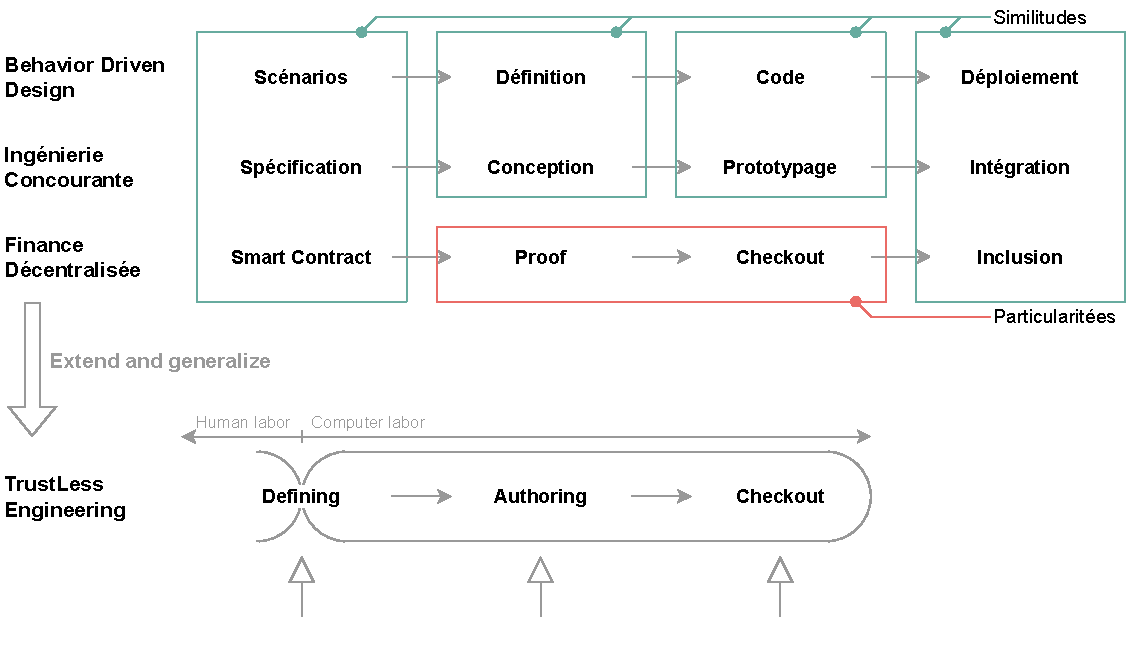
\includegraphics[width=.9\linewidth]{./svg/long-term-goal.pdf}
\caption{\label{fig:org367db3a}Vers une ingénierie sans confiance ?}
\end{figure}
\subsubsection{Améliorations techniques}
\label{sec:org97143dd}
\subsubsection{Extensions domaines}
\label{sec:org8927ee6}
\subsection{Impact scientifique et industriel}
\label{sec:org014e786}
\subsubsection{Impact sur la recherche}
\label{sec:org828e6d4}
\subsubsection{Impact industriel}
\label{sec:org6d0a937}
\subsubsection{Impact sociétal}
\label{sec:orgc7bae30}
\clearpage
\section{Conclusion générale}
\label{sec:org81ad99b}
Synthèse des contributions

Contribution théorique majeure

Innovation méthodologique

Validation expérimentale

Réponse à la question principale

Réponse à la questions secondaires

Perspectives d'avenir


\begin{quote}
{[}!Info] Commentaire prospectif sur l'ouvrage et ses conclusions
\end{quote}

Espérer une évolution des plateformes d'accès aux normes (cobaz) pour simplifier la configuration des environnements de travail (NF EN etc. et gestion des exigences)

L'avenir, un terrain fertile pour l'ingénierie intégrée ?

Les futures ruptures technologiques (?)
\clearpage
\section{Références du document}
\label{sec:org5f3c891}
\subsection{Liste des figures}
\label{sec:orgb492da0}
\renewcommand{\listfigurename}{\vspace{-2em}}
\listoffigures
\subsection{Liste des tableaux}
\label{sec:org264ec1d}
\renewcommand{\listtablename}{\vspace{-2em}}
\listoftables
\subsection{Liste des codes sources}
\label{sec:orgeda376e}
\renewcommand{\lstlistingname}{\vspace{-2em}}
\listoflistings
\subsection{Liste des glosses}
\label{sec:org1e91abb}


\subsection{Liste des acronymes}
\label{sec:orgadc2b45}

\clearpage
\section{Bibliographie}
\label{sec:orgc9b20d6}
\printbibliography[heading=none]

\clearpage

\appendix
\section{Analyse des normes}
\label{sec:orgde0bd1c}
\subsection{Introduction}
\label{sec:org41da8ca}
\subsection{Périmètre de l'étude}
\label{sec:org7cf6c5d}
L’étude se concentre sur les normes volontaires françaises (NF) référencées par AFNOR et publiées à la date de la collecte.
Le périmètre inclut toutes les normes relevant du domaine “Construction et urbanisme” selon la classification AFNOR Norm’Info.

Les normes ISO/IEC sont souvent transposées en normes NF (NF EN ISO, etc.)

AFNOR est le point d’entrée national reconnu par l’État pour la normalisation volontaire.

Les normes d’application obligatoire sont issues de ce corpus (via réglementations).

Par l'analyse des textes et de leurs métadonnées, nous tenterons de répondre aux questions suivantes :

Q1 : Quelle est l’ampleur documentaire du corpus normatif applicable à l’industrie de la construction, mesurée en nombre de documents et en volume paginé ?
Q2 : La filière construction présente-t-elle une densité normative supérieure à celle d’autres secteurs industriels comparables, en termes de nombre de normes actives et de leur volumétrie documentaire ?
Q3 : Comment les textes normatifs se répartissent-ils entre les sous-domaines techniques, professions et spécialités représentatives de la filière construction, selon les descripteurs et indices de classement ?
\subsection{Méthodologie}
\label{sec:orgeb0ca00}
\subsubsection{Cadre juridique}
\label{sec:org42a6fc5}
Il n'existe pas de base de données publiques recenssant l'ensemble des textes de normes et leurs métadonnées. Il convient donc de constituer cette base de donnée en collectant les informations publiquement accessibles.

Cette opération implique l'emplois du webscraping.

\begin{quote}
Le webscraping consiste à extraire automatiquement (to scrape : gratter), de manière massive des données d'un site web. -- INRAE\autocite{quesnevilleRecommandationsUsagesWebscraping2024}
\end{quote}

La légalité d'une telle opération semble parfois faire débat. (ref à ajouter)

En droit français, le Code de la propriété intellectuelle précise les modalités de copie et de reproduction des bases de données :
\begin{quote}
Lorsqu'une base de données est mise à la disposition du public par le titulaire des droits, celui-ci ne peut interdire :

{[}\ldots{}]

6° Les extractions, copies ou reproductions numériques d'une base de données, en vue de la fouille de textes et de données réalisée dans les conditions prévues à l'article L. 122-5-3. Pour l'application de cet article, les auteurs et titulaires des droits d'auteur s'entendent des producteurs de bases de données et les copies ou reproductions numériques d'œuvres s'entendent des extractions, copies ou reproductions numériques de bases de données ;

-- Article L342-3\autocite{CodeProprieteIntellectuelle}
\end{quote}

Ce code précise également les droits de manipulation des textes dans un cadre de recherche :
\begin{quote}
Lorsque l'oeuvre a été divulguée, l'auteur ne peut interdire :

{[}\ldots{}]

10° Les copies ou reproductions numériques d'une œuvre en vue de la fouille de textes et de données réalisée dans les conditions prévues à l'article L. 122-5-3 ;

-- Article L122-5\autocite{CodeProprieteIntellectuelle}
\end{quote}

Et :
\begin{quote}
I.-On entend par fouille de textes et de données, au sens du 10° de l'article L. 122-5, la mise en œuvre d'une technique d'analyse automatisée de textes et données sous forme numérique afin d'en dégager des informations, notamment des constantes, des tendances et des corrélations.

II.-Des copies ou reproductions numériques d'œuvres auxquelles il a été accédé de manière licite peuvent être réalisées sans autorisation des auteurs en vue de fouilles de textes et de données menées à bien aux seules fins de la recherche scientifique par les organismes de recherche, les bibliothèques accessibles au public, les musées, les services d'archives ou les institutions dépositaires du patrimoine cinématographique, audiovisuel ou sonore, ou pour leur compte et à leur demande par d'autres personnes, y compris dans le cadre d'un partenariat sans but lucratif avec des acteurs privés.

{[}\ldots{}]

Les copies et reproductions numériques effectuées lors d'une fouille de textes et de données sont stockées avec un niveau de sécurité approprié et peuvent être conservées à des fins exclusives de recherche scientifique, y compris pour la vérification des résultats de la recherche.

-- Article L122-5-3\autocite{CodeProprieteIntellectuelle}
\end{quote}
\subsubsection{Données collectées}
\label{sec:org4ffa4f4}
Métadonnées accessibles publiquement via Norm’Info et Boutique AFNOR :
    Référence (ex : NF C15-100)
    Titre
    Date de publication
    Nombre de pages
    Codes ICS
    Indice de classement
    Domaine technique
    Commission de normalisation
\subsubsection{Protocole technique}
\label{sec:orgefde17d}
Méthode de collecte : Web scraping (à documenter)

Limite : seules les normes publiées et publiquement référencées sur le site marchand de l'AFNOR disponibles à la vente ou référencées, sont incluses.
\subsection{Méthodes d'analyse}
\label{sec:org407699a}
Analyse descriptive :
    Nombre total de documents / pages
    Évolution temporelle des publications (si date disponible)

Analyse comparative :
    Densité normative dans la construction vs autres domaines AFNOR (en comparant les volumes ICS sectoriels)

Analyse thématique / taxonomique :
    Catégorisation des normes par code ICS, indice de classement, domaine technique
    Projection possible par métier : architecture, génie civil, thermique, électricité…

Outils recommandés : Python (pandas + matplotlib)
\subsection{Résultats obtenus}
\label{sec:org023784a}
Cartographie de la norme dans la construction

Poids normatif par spécialité

Identification d’une sur-normativité éventuelle

Premiers indicateurs pour évaluer la « charge de la norme »
\subsection{Discussion et perspectives}
\label{sec:org871d87e}
\clearpage

\end{document}
\end{document}
